% Chapter Template

\chapter{System Design and Architecture}\doublespacing % Main chapter title

\label{Chapter5} % Change X to a consecutive number; for referencing this chapter elsewhere, use \ref{ChapterX}

\lhead{Chapter V. \emph{System Design and Architecture}} % Change X to a consecutive number; this is for the header on each page - perhaps a shortened title


% --------------------------------
% Study Summary
% --------------------------------

\section{Introduction}
\noindent The system design and architecture are of utmost importance when it comes to the implementation of a supply chain management system using blockchain technology. A well-designed system ensures the efficient and secure management of the supply chain, leveraging the unique capabilities offered by blockchain.
To effectively design the system architecture for a blockchain-based supply chain management system, several key aspects need to be considered. These include:

% ----------------------------
% Conclusions
% ----------------------------

\subsection{Hyperledger Fabric}
\noindent The Fabric network comprises three organizations (Manufacturer, Middle Men, and Consumer) with five peers, one orderer, and one channel. Each organization has its own Fabric CA for managing digital certificates. The network uses Fabric CA as the Certificate Authority for secure authentication and authorization. The peers maintain a copy of the shared ledger and execute chaincode for smart contracts. The Orderer validates and orders transactions, ensuring consistency. The Fabric network with Fabric CA provides a secure, transparent, and efficient solution for managing the operations.
% \begin{figure}[ht]
\centering
\begin{minipage}[b]{\linewidth}
  \centering
  \includegraphics[width=0.4\linewidth]{Chapters/Chapter_3/figures/Image3_1a.PNG}
  \subcaption{Plot1 with a single image (Image by pencil parker from Pixabay)}
\end{minipage}

\begin{minipage}[b]{\linewidth}
  \centering
  \includegraphics[width=0.4\linewidth]{Chapters/Chapter_3/figures/Image3_1b.PNG}
  \subcaption{Plot2 with a single image (Image by pencil parker from Pixabay)}
\end{minipage}
\caption{Main caption}
\label{fig:figure3_1}
\end{figure}









\begin{figure}[htbp]
  \centering
  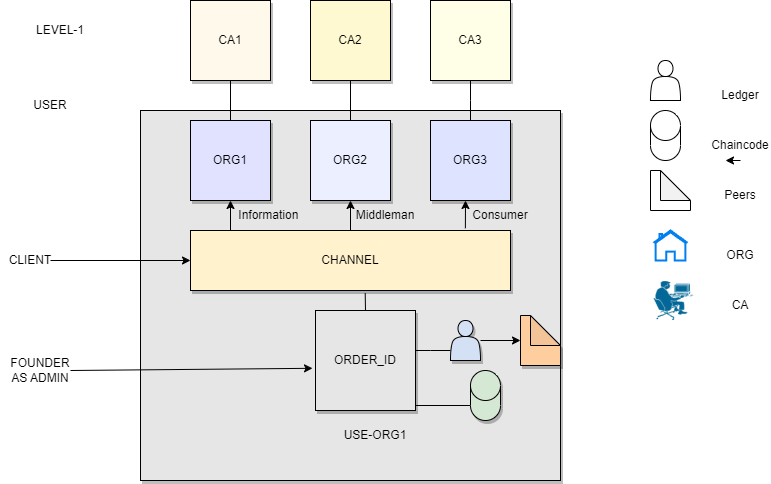
\includegraphics[width=0.9\textwidth]{Chapters/Chapter_5/figures/figure5_1.png}
  \caption{Hyperledger Fabric network Architecture }
  \label{fig:figure5_1}
  \end{figure}

\noindent The Fabric network comprises three organizations (Manufacturer, Middle Men, and Consumer) with five peers, one orderer, 
and one channel. Each organization has its own Fabric CA for managing digital certificates. The network uses Fabric CA as 
the Certificate Authority for secure authentication and authorization. The peers maintain a copy of the shared ledger and 
execute chain code for smart contracts. The Orderer validates and orders transactions, ensuring consistency. The Fabric 
network with Fabric CA provides a secure, transparent, and efficient solution for managing operations.

\begin{itemize}
  \item Admin: all the organization.
  \item Manufacturer: Org1.
  \item Middleman: Org2.
  \item Consumer: Org3.
\end{itemize}
    
% ----------------------------
% Scope for Future Work
% ----------------------------

\subsection{Membership and Access Control}
\begin{figure}[htbp]
  \centering
  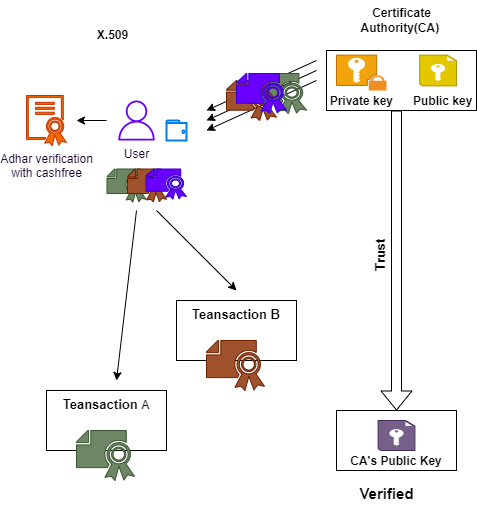
\includegraphics[width=0.9\textwidth]{Chapters/Chapter_5/figures/x.509.png}
  \caption{X.509 Identity Management }
  \label{fig:figure5_2}
  \end{figure}
\noindent \ref{fig:figure5_2} shows that there is a CA that issues a certificate to the user, and this X.059 certificate has multiple attributes whenever 
the user performs a transaction, it signs using this certificate and also checks for Aadhar verification status. Any other entity 
in the system that can view these transactions will be able to see their attributes, thereby knowing that the transaction was 
performed by the particular user to ensure trustworthy of each user in the network.

\subsection{Machine Learning}
\noindent 
The developed solution presents a machine learning (ML) model for detecting the freshness of fruits using a Convolutional Neural Network (CNN) algorithm. The model is trained using TensorFlow, an open-source library for deep learning and machine learning tasks, and is supported by other libraries such as NumPy, Pandas, and Matplotlib for data handling, data cleaning, and visualization. The dataset used for training the model is imported, and its length is verified to be 10901. The model is trained with a sequential model using different layers, including convolutional, activation, dropout, max pooling, flattening, and dense, each serving a specific function in the training process. Keras, a popular library for building neural networks, is used to create the final layers of the CNN model.
\par The model is compiled with the RMSprop optimizer, a commonly used optimizer in ML models. During training, the data is traversed multiple times using epochs, with an epoch value of 100 in this case. A validation-data of validation-generator with verbose 2 used  in the model training process. The proposed approach combines various libraries, algorithms, and tools to develop an ML model for detecting the freshness of fruits based on their condition, which can be beneficial in tracking the quality of products in supply chains. The solution contributes to the expanding body of literature on blockchain applications by providing an effective, dependable, secure, and decentralized trace and track solution using ML and blockchain technologies.
\begin{figure}[ht]
  \centering
  \begin{minipage}[b]{0.4\linewidth}
    \centering
    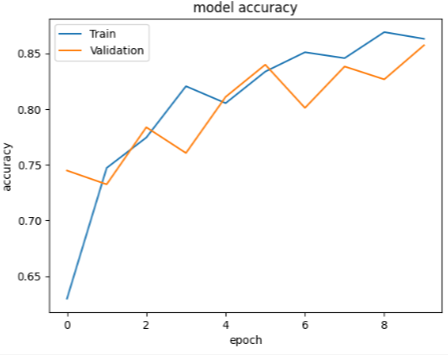
\includegraphics[width=\linewidth]{Chapters/Chapter_5/figures/model_accurecy.png}
    \subcaption{Model Accurecy}
  \end{minipage}
  \hfill
  \begin{minipage}[b]{0.4\linewidth}
    \centering
    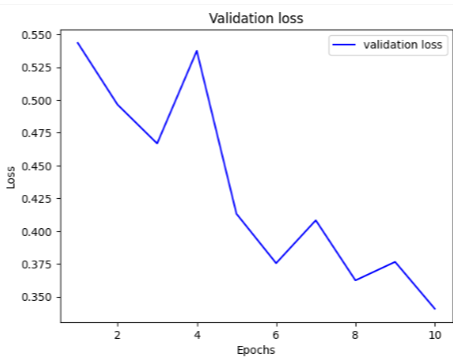
\includegraphics[width=\linewidth]{Chapters/Chapter_5/figures/validationloss.png}
    \subcaption{Validation loss}
  \end{minipage}
  \caption{Main caption}
  \label{fig:figure5_3}
  \end{figure}
  
  % \begin{figure}[ht]
  %   \centering
  %   \begin{minipage}[b]{0.7\linewidth}
  %     \centering
  %     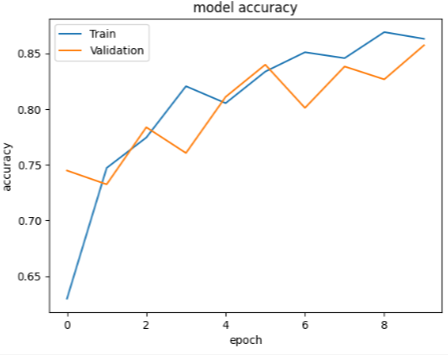
\includegraphics[width=\linewidth]{Chapters/Chapter_5/figures/model_accurecy.png}
  %     \subcaption{Model Accuracy}
  %   \end{minipage}
  
  %   \vspace{0.5cm} % Adjust the vertical space between the images
  
  %   \begin{minipage}[b]{0.4\linewidth}
  %     \centering
  %     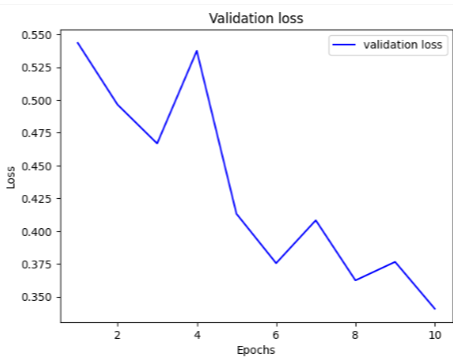
\includegraphics[width=\linewidth]{Chapters/Chapter_5/figures/validationloss.png}
  %     \subcaption{Validation Loss}
  %   \end{minipage}
    
  %   \caption{Main Caption}
  %   \label{fig:figure5_3}
  % \end{figure}
  
  
  
  
  
  
  
\noindent \ref{fig:figure5_3} (a) shows the training accuracy and Validation accucy.Train graph shows the overall model’s Training accuracy and validation accuracy shows the Subset of the training data .It is seen that with each epoch Model is giving more accuracy also validation accuracy too. Validation accuracy is calculated by using subset of the whole 
Training dataset.The final accuracy of the Model is found to be 91.5\%.
\ref{fig:figure5_3} (b) shows the output result that our model  provides.It can be seen That our model is providing us the correct
output.For a rotten Fruit it predicts the fruit as rotten and for a fresh it predicts as fresh.

\subsection{Webapp}
\begin{figure}[ht]
    \centering
    \begin{minipage}[b]{\linewidth}
      \centering
      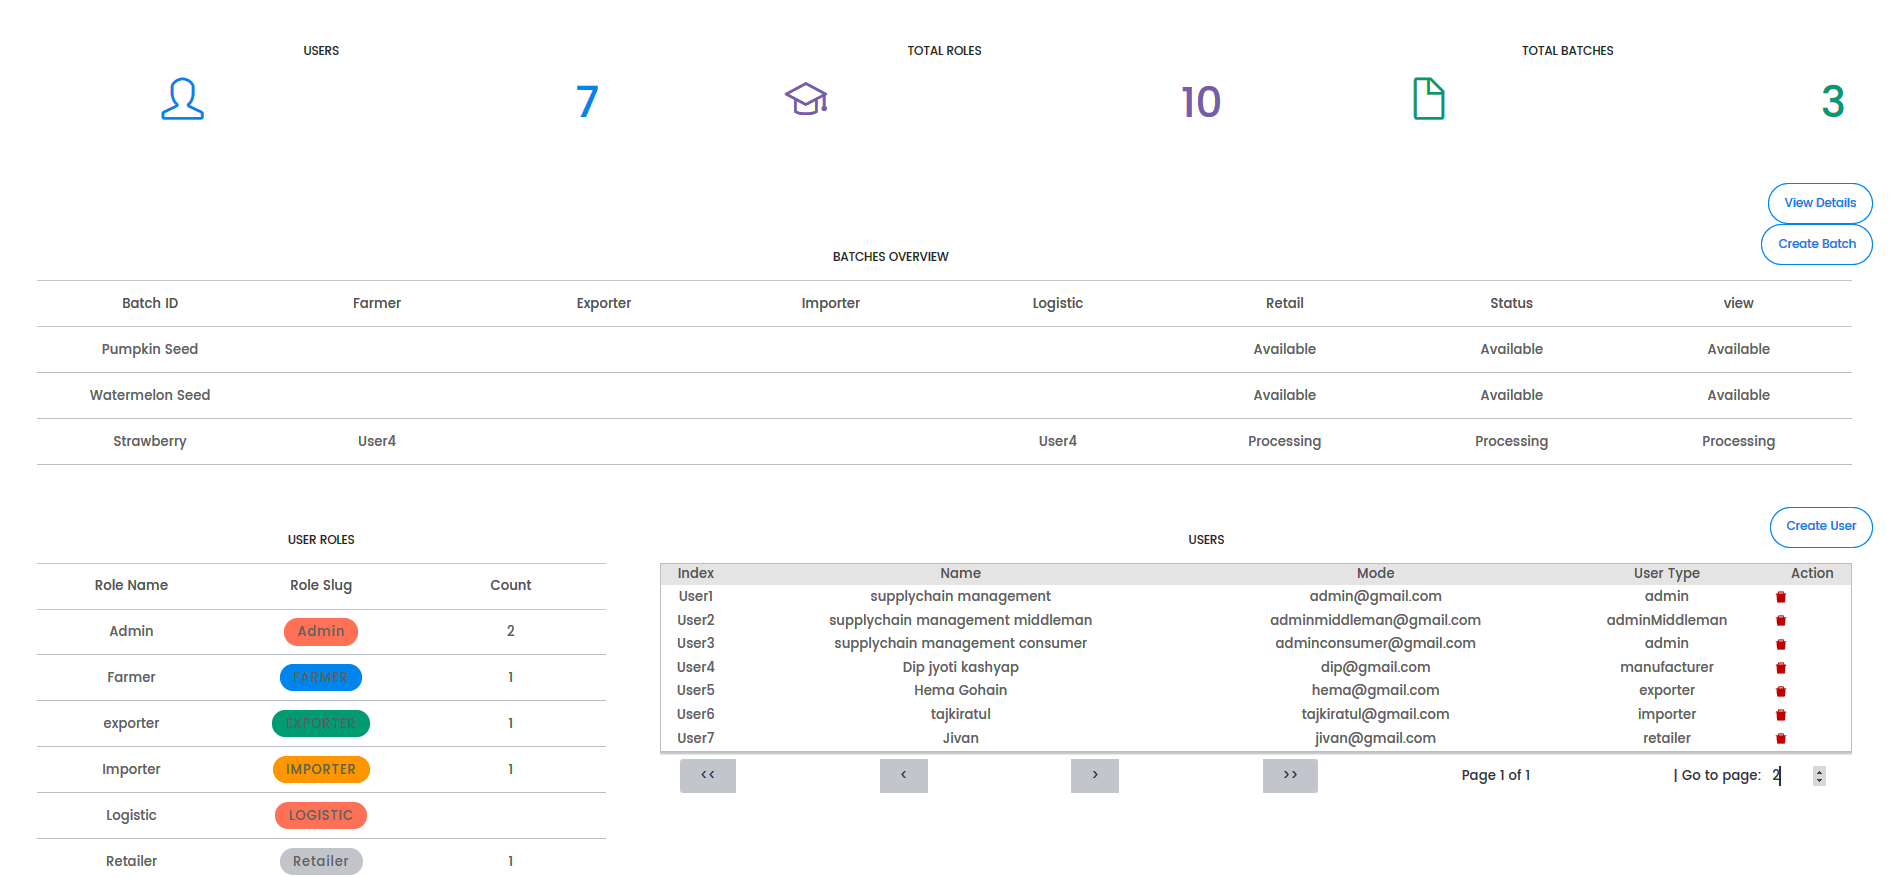
\includegraphics[width=\linewidth]{Chapters/Chapter_5/figures/dashboard.png}
      \subcaption{Admin Dashboard}
    \end{minipage}
    \hfill
    \begin{minipage}[b]{\linewidth}
      \centering
      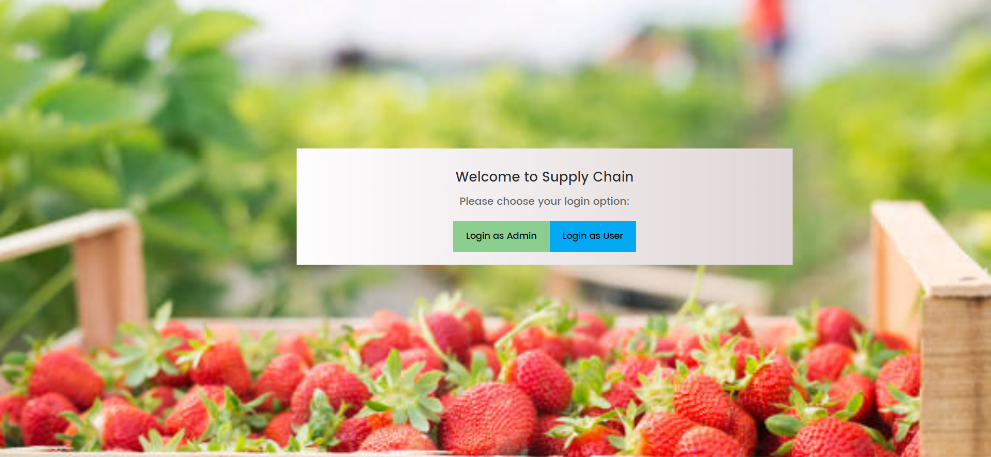
\includegraphics[width=\linewidth]{Chapters/Chapter_5/figures/login.png}
      \subcaption{Login Screen}
    \end{minipage}
    \caption{Main caption}
    \label{fig:figure5_4}
    \end{figure}

\noindent The frontend application is developed using React.js, providing a user-friendly interface for capturing product images, interacting with the supply chain system, and receiving real-time quality predictions. The application allows authorized participants to capture product images using a camera and sends transaction proposals to the appropriate peers in the Hyperledger Fabric network for further processing.

\subsection{REST API Layer}
\noindent shows the API endpoints build using express.js implemented using Node.js to handle requests and responses between the frontend application and the Hyperledger Fabric network. The APIs facilitate the communication between the frontend application and the smart contracts deployed on the peers for transaction submission, endorsement, and validation such as managing users, goods, orders, and asset tracking, asset transfer which are part of the Supply Chain Management Chaincode.
The ``Admin" role is intended to utilize the ``createUser" method to add new users to the system. Users can log in and authenticate their credentials using the ``sign in" feature.
The ``Manufacturer" role has access to the ``createProduct" method, which lets them add new goods to the blockchain. The ``Manufacturer" ``Exporter" ``Importer" and ``Retailer" roles can change a product's information and status as it passes through the supply chain by using the ``update product" function.
As items are delivered from one supply chain entity to another, the functions ``sendToExporter" ``sendToImporter" and ``sendToRetailer" are used to update the asset transfer status of those products.
Then at last a consumer can buy the product from a retailer.

\section{Proposed system}
\begin{figure}[htbp]
    \centering
    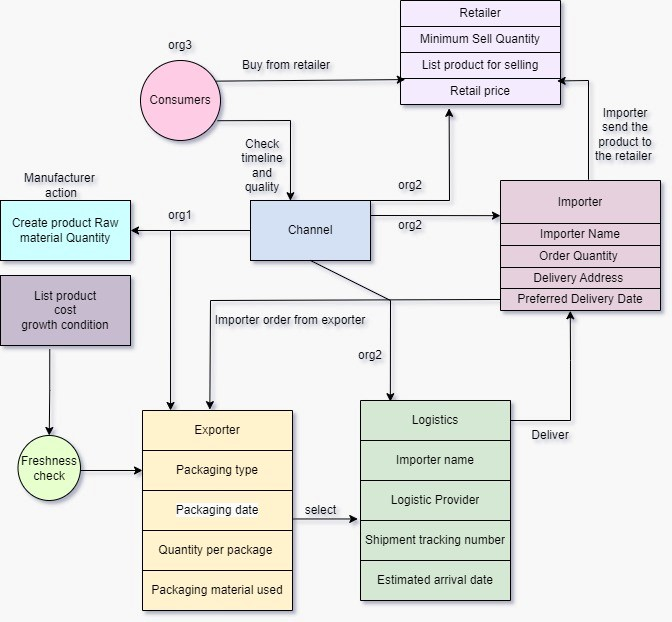
\includegraphics[width=0.9\textwidth]{Chapters/Chapter_5/figures/data_flow.jpg}
    \caption{Class Diagram}
    \label{fig:figure5_5}
    \end{figure}
\noindent The details of the participation of the network are displayed in Figure 10. Each participant has a unique identity number in the network that is generated by the system using which a participant can participate in the network and each asset has its own unique identity to identify and process at each stage. Also, some additional attributes vary according to the nature of the product and stage.

\begin{figure}[htbp]
    \centering
    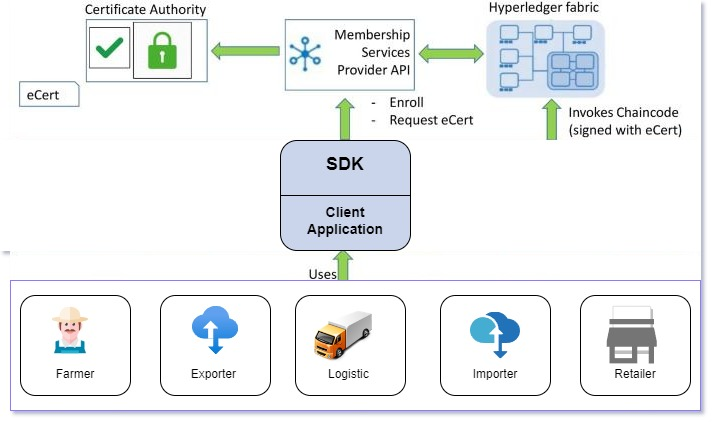
\includegraphics[width=0.9\textwidth]{Chapters/Chapter_5/figures/proposed_system.png}
    \caption{proposed system Architecture }
    \label{fig:figure5_6}
    \end{figure}
\noindent shows our proposed architecture using hyper ledger fabric and an ML model that checks the quality of the product before passing it to the next participant. Each participant is interconnected and each of them maintains a peer along with the ledger in their given organization. Each participant has to take a membership and later be verified by Aadhar to participate in the network. The membership service provider issues certificates, ECert (Enrollment Certificates), through the CA (Certificate Authority) to the requested peers. These certificates act as identities for the peers. To execute transactions in the Hyperledger Fabric environment, chaincode procedures are called. Chaincode procedures are initiated by any authenticated peer and executed by all peers in the network.

\subsection{Product Management}
\indent The proposed system is simulated by product management and verification. where a product with a unique identification id and credential contains all the information about its producer, manufacturer, importer, exporter, and retailer.
and its management is achieved by creating product update products and querying products.
\begin{itemize} 
\item	Admin is in charge of generating user accounts and authorizing access to the system, as well as enrolling people in the network, Manufacturer is allowed to generate new ones within the system.
\item	The exporter, who serves as a middleman in the supply chain, receives a new product once it is made by the Manufacturer. The Exporter is in charge of getting the item from the Manufacturer and getting it to the Importer, who is the next supply chain participant.
\item	 The importer is in charge of delivering the goods to the Retailer, who is the following party in the supply chain, after receiving it from the Exporter. 
\item	Logistics is in charing of carrying out the shipment and delivery of the product from one participant to another.
\item	The retailer is responsible for selling the product to the end consumer, who can place an order for the desired product.
\end{itemize}
\indent Once the product is delivered to the consumer, they can mark it as ``Delivered" in the system, indicating that the product has been received. This helps in tracking the status of the product delivery and ensures transparency and accountability in the supply chain process.
At each step of the supply chain, the ML model check the product's condition and quality and if it's found to be damaged then the product is rejected and it will not move to the next step of the supply chain.
